%Template v.1.0: Taylor Arnold and Simon Gabay, december 2025
% CECI EST UN FICHIER DE MODÈLE LATEX POUR LES ARTICLES INCLUS DANS
% *Anthology of Computers and the Humanities*. AJOUTEZ L'OPTION
% 'final' LORS DE LA CRÉATION DE LA VERSION FINALE DE L'ARTICLE. 
% NE PAS modifier la classe du document
%\documentclass[final, fra, custom]{anthology-ch}     % pour la version finale
\documentclass[fra, final]{anthology-ch}      % pour la soumission

% CHARGER LES PACKAGES LaTeX
\usepackage{booktabs}
\usepackage{graphicx}
\usepackage{wrapfig} % pour les figures dans le §
% AJOUTEZ vos propres packages avec \usepackage{}

% TITRE DE LA SOUMISSION
% Remplacez ceci par le titre de votre soumission
\title{Concerts et itinéraires: spatialiser le free jazz en Europe d'après \textit{Jazz Hot} (1966-1976)}

% INFORMATIONS SUR LES AUTEURS ET LES AFFILIATIONS
% Pour chaque auteur, utilisez une nouvelle commande \author, avec
% les numéros entre crochets indiquant les affiliations correspondantes
% (section suivante) et l'ORCID-ID pour chaque auteur.  
\author[1]{Thomas Gauffroy-Naudin}[
orcid=0009-0003-5309-8515,
email=Thomas.Gauffroy-Naudin@unige.ch
]

% Bien que nous encouragions l'ajout des ORCID-ID pour tous les auteurs, 
% vous pouvez inclure des auteurs qui n'en ont pas en laissant le champ vide.

% Il doit y avoir un appel à \affiliation pour chaque affiliation des auteurs.
% Plusieurs affiliations peuvent être attribuées à un auteur
% et une affiliation peut être attribuée à plusieurs auteurs. 
\affiliation{1}{Université de Genève, Suisse}
\affiliation{2}{Music and Migration Lab, New York, United-States}

% MOTS-CLÉS
% Fournissez un ou plusieurs mots-clés séparés par des virgules
% en utilisant les commandes suivantes
\keywords[fra]{Free jazz, OCR, diaspora jazz, cartographie, \textit{Jazz Hot}, circulation culturelle, Europe du XXe siècle}
\keywords[eng]{Free jazz, OCR, jazz diaspora, mapping, \textit{Jazz Hot}, cultural circulation, 20th century Europe}

% MÉTADONNÉES DE LA PUBLICATION
% Ces champs seront remplis lors de la publication ; 
% ils peuvent être laissés par défaut lors de la soumission
\pubyear{2026}
\pubvolume{4}
\pagestart{63}
\pageend{71}
\paperorder{8}
\conferencename{Actes de la Conférence Humanistica}
\conferenceeditors{Serena Crespi, Simon Gabay, Martin Grandjean, Ariane Pinche, Marie Puren et Léa Saint-Raymond}
\doi{10.63744/ildDkDLhsZu5}
\customhead{}

\addbibresource{bibliography.bib}

%%%%%%%%%%%%%%%%%%%%%%%%%%%%%%%%%%%%%%%%%%%%%%%%%%%%%%%%%%%%%%%%%%%%%%%%%%%
% DÉBUT DU TEXTE
\begin{document}
	
	\maketitle
	
	\begin{abstract}
		By the mid-1960s, the free jazz movement had expanded beyond New York, and Europe became a destination for a new stream of American musicians. The French jazz press, by systematically documenting concerts and festivals, provides a valuable resource for tracing these movements and examining the dynamics of jazz’s globalization. This work aims to map the performance venues and free jazz artist's routes across western Europe based on an analysis of \textbackslash{}textit\{Jazz Hot\} from 1966 through 1976. The prototype pipeline thus resorts to a fine tuned OCR model to extract performance references, which are then georeferenced and mapped on a dedicated platform with aim to shed light on the geographical distribution of free jazz. \end{abstract}
	
	\section{Introduction}
	L'Europe constitue, selon les termes de Joël Pailhé, l'un des pôles d'un « oligopole mondial du jazz » aux côtés des États-Unis et du Japon \cite{pailhe_jazz_1998}. À ce titre, elle offre un terrain d'observation privilégié pour étudier la mondialisation du jazz durant la décennie free. L'arrivée massive de musiciens américains à Paris à partir de 1969 répond d'abord à des logiques économiques liées au déclin du marché américain, mais prolonge aussi une tradition d'accueil des artistes afro-américains remontant à l'entre-deux-guerres \cite{drott_free_2008}.
	
	Pourtant, si le jazz circule désormais bien au-delà du lieu qui l'a vu naître, les déplacements de ses musiciens en Europe restent mal documentés. Dans ce contexte, la presse jazz est une ressource précieuse où les programmes de concerts, rubriques d'actualité et critiques nous renseignent sur les dates, les lieux et les artistes qui se produisent sur ce continent. Ces périodiques constituent ainsi des index partiels des mouvements d'artistes et témoignent de la dynamique du paysage artistique du jazz. 
	
	Le présent travail vise à exploiter cette documentation pour cartographier les flux de jazzmen en Europe. La source principale est la revue Jazz Hot, fondée en 1935, qui occupe une position centrale dans le champ français du jazz \cite{roueff_espace_2019}. Notre démarche consiste à extraire systématiquement les mentions de performances scéniques, à géolocaliser les lieux de concert, puis à reconstituer les trajets entre destinations pour faire apparaître les circuits de diffusion.
	
	
	\section{État de l'art}

	Les recherches existantes sur la diffusion du jazz en Europe proposent surtout des études de cas individuels et prosopographiques  \cite{clark_making_2017,ross_jazz_2000,braggs_jazz_2016}, ou sur sa réception critique \cite{sklower_rebel_2008,roueff_espace_2019}, et sa politisation \cite{drott_free_2008,le_texier_critique_2018}. Si ces travaux sociologiques et historiques fournissent un cadre indispensable, ils pourraient bénéficier d'analyses quantitatives basées sur des données. Un premier pas vers cette approche se trouve dans le travail de Joël Pailhé, qui établit un indice de diffusion du jazz en Europe à partir du cumul de chaînes de radios, de revues spécialisées, de festivals et de musiciens recensés dans chaque pays \cite{pailhe_jazz_1998}.
	
	Plus récemment, plusieurs projets de cartographie numérique ont ouvert la voie à une analyse plus distante. La plateforme \textit{Free Jazz NYC} propose ainsi une cartographie dans le temps (\textit{timeline}) des lieux de représentation du free jazz à Manhattan\footnote{\url{https://freejazz.nyc/index}.}, tandis que l'application \textit{Jazz Venues} spatialise les clubs de jazz parisiens des années 1920  \footnote{\url{https://musicalgeography.org/project/jazz-venues}.}. Sur la question spécifique des déplacements d'artistes, \textit{The Travels of Josephine Baker and Sidney Bechet} démontre le potentiel de la cartographie d'itinéraires \footnote{\url{https://musicalgeography.org/project/the-travels-of-josephine-baker-and-sidney-bechet}.}. Toutefois, ces projets restent limités dans leurs corpus et aucun n'a étudié des périodiques en masse grâce à des outils HTR.
	
	Nous nous tournons plutôt vers le projet BasArt \footnote{\url{https://artlas.huma-num.fr/map}.} comme référence en matière de base de données interactive sur la circulation d'artistes à partir d'imprimés \cite{de_maupeou_cartographie_2012}. C'est cette approche, notamment dans le traitement des sources et la structuration des données, qui nous semble la plus propice au développement d'une plateforme à grande échelle.
	
	
	\section{Entraînement du modèle OCR}
	
	\subsection{Données}
	
	\begin{wraptable}{r}{0.5\textwidth}
		\centering
		\vspace{-.4cm}
		\resizebox{1\linewidth}{!}{
			\begin{tabular}{l|ccc}
				\toprule
				\textbf{ID} &  \textbf{Nombre de} &\textbf{Nombre}&\textbf{Échantillons}\\
				&  \textbf{numeros} &\textbf{de vues}&\textbf{}\\
				\midrule
				JH\_1966&8&42&4\\
				JH\_1967&1&7&5\\
				JH\_1968&4&25&10\\
				JH\_1969&2&16&9\\
				JH\_1970&11&66&5\\
				JH\_1971&11&57&2\\
				JH\_1972&11&41&3\\
				JH\_1973&11&35&6\\
				JH\_1974&10&30&4\\
				JH\_1975&11&48&4\\
				JH\_1976&11&37&3\\
				\midrule
				\textbf{Total}&  91 &404&55\\
				\bottomrule
			\end{tabular}
		}
		\caption{Corpus complet et échantillons pour l’entraînement du modèle OCR.}
		\label{tab:full_corpus}
		\vspace{-.5cm}
	\end{wraptable}
	Le premier défi consiste à rassembler suffisamment de sources pour constituer un jeu de données complet. Le manque d'intérêt pour la numérisation de la presse jazz explique la difficulté à localiser des numéros de \textit{Jazz Hot}. Bien qu'une collection de revues européennes de jazz existe au \textit{Centro Nazionale Studi sul Jazz} à Sienne \footnote{\url{https://centrostudi.sienajazz.it/archivio/archivio-riviste}}, l'absence de données accessibles en ligne et le coût de la numérisation ont conduit ce projet à former un corpus à partir de notre collection personnelle de revues. De par ces limites, notre sélection contient moins de données pour les années 1966 à 1970. Une seconde contrainte à l'accessibilité des données tient au statut juridique de la revue qui est soumise au droit d'auteur et donc non distribuable librement. 
	
	Notre corpus d'entraînement se compose d'un échantillon de 55 pages sélectionnées en fonction de l’intérêt pour les rubriques pouvant mentionner des concerts (actualités, programmes, critiques). Le déséquilibre de l’échantillonnage se justifie par une large variation typographique selon les numéros. En effet, ceux de 1968 et 1969 sont davantage représentés en raison de changements de mise en page et de police plus fréquents durant cette période, tandis que les numéros des années 1970 sont plus homogènes dans leur typographie.
	
	\subsection{Analyse de mise en page}
	Les pages sélectionnées ont été segmentées manuellement à l'aide de FoNDUE, une instance d'eScriptorium de l'Université de Genève \cite{noauthor_escriptorium_nodate} utilisant Kraken (v5.3.0)  \cite{noauthor_kraken_nodate}. Puisque le projet se limite à l'extraction de données précises dans le corps du texte (noms, dates et lieux), une segmentation fine de l'image n'est pas nécessaire. La structure en colonnes du magazine nécessite un traitement adapté pour assurer la bonne détection des lignes. Nous reprenons ainsi des préconisations du projet SegmOnto \cite{gabay_segmonto_2024} et distinguons les zones suivantes :
	
	\begin{figure}[!ht]
		\centering
		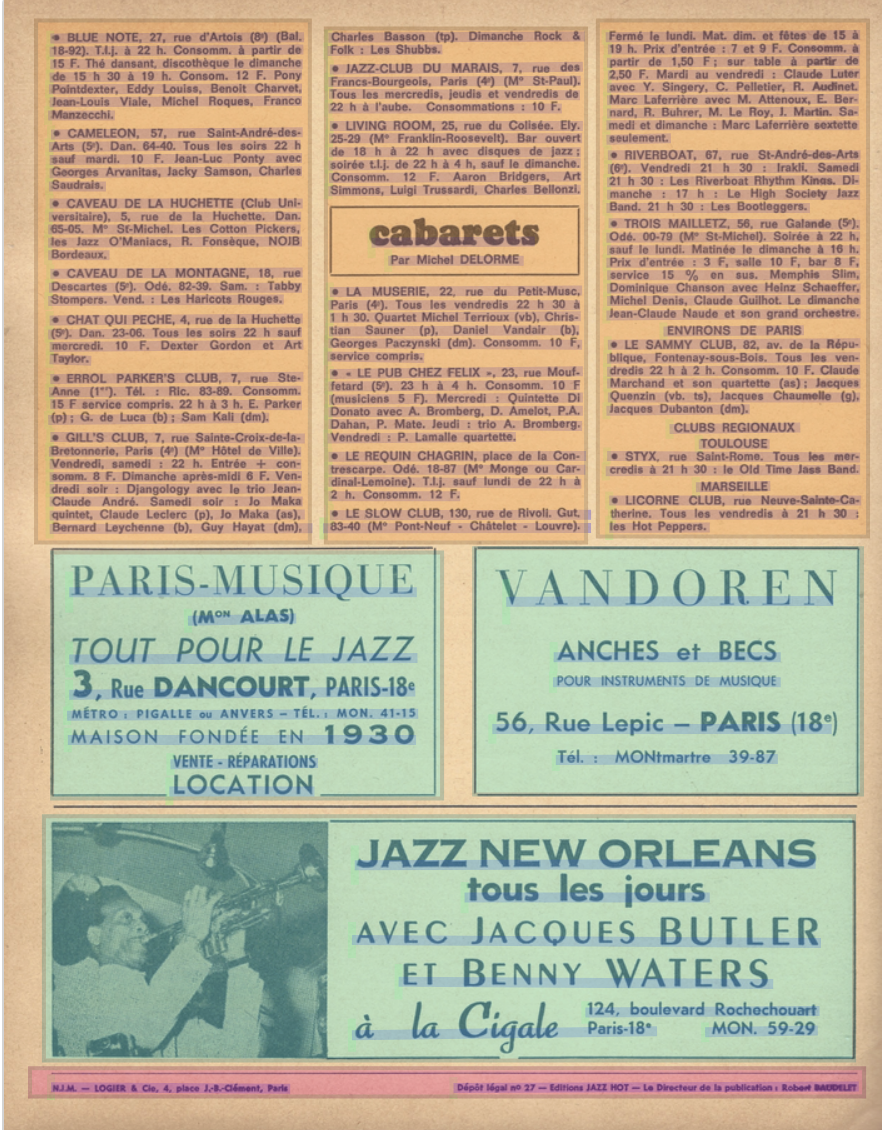
\includegraphics[width=\linewidth]{Figure_1_Sementation.png}
		\caption{JH\_67\_04 \texttt{MainZone} (jaune), \texttt{AdvertisementZone:} (vert), \texttt{TextZone} (rouge).}
		\label{fig:jazzhot_segmentation}
	\end{figure}
	
	\begin{itemize}
		\item \textbf{\texttt{AdvertisementZone}:}  zone personnalisée pour les publicités
		\item \textbf{\texttt{GraphicZone}:} images (hors publicités)
		\item \textbf{\texttt{MainZone}:} une par colonne (données pertinentes)
		\item \textbf{\texttt{NumberingZone}:} numéro de page
		\item \textbf{\texttt{TextZone}:} textes divers et légendes
		\item \textbf{\texttt{TitlePageZone}:} titres de rubriques
	\end{itemize}
	
	\noindent L'ensemble des lignes est étiqueté \texttt{DefaultLine}.

Un modèle de segmentation automatique a été entraîné à partir de ces données mais les résultats restent insuffisants pour être exploités en l'état.
	
	
	\subsection{Transcription}
	\begin{wraptable}{r}{0.5\textwidth}
		\centering
		\vspace{-.4cm}
		\resizebox{1\linewidth}{!}{
			\begin{tabular}{lcll}
				\toprule
				\textbf{Catégorie}& \textbf{Cas}& \textbf{Traitement} &\textbf{Exemple}\\
				\midrule
				Listes& Puce& Conservation& 
\includegraphics[width=2cm]{exemple_puce.png}\\
				& & U+2022 (‹•›)&\\
			\end{tabular}
		}
		\caption{Règle de transcription pour les puces.}
		\label{tab:transcription_guideline}
        \vspace{-.3cm}
	\end{wraptable}
	En l’absence d'un guide spécifiquement dédié aux magazines imprimés du XX\ieme{}~siècle, nous suivons les recommandations de CATMuS \textit{Print} pour la transcription des données \cite{gabay_catmus-print_2024,gabay:hal-04557457}. Toutefois, ces préconisations ne couvrent pas les puces, pourtant récurrentes dans nos sources. Le modèle CATMuS \textit{Print} [large] les détectant déjà correctement, nous avons choisi de les conserver pour améliorer cette reconnaissance (Tab.~\ref{tab:transcription_guideline}).
	
	\begin{wraptable}{r}{0.5\textwidth}
		\centering
		\vspace{-.4cm}
		\resizebox{1\linewidth}{!}{
			\begin{tabular}{lc}
				\toprule
				\textbf{Modèle}& \textbf{Character Accuracy}\\
				\midrule
				Catmus-print-fondue-large& 98.03\%\\
				Catmus-JH& \textbf{98.73\%}\\
				\bottomrule
			\end{tabular}
		}
		\caption{Résultat de l’évaluation sur un échantillon de 11 images.}
		\label{tab:OCR_model_score}
        \vspace{-.3cm}
	\end{wraptable}
	
	\subsection{Modèles}
	Les données d’entraînement ont d'abord été prétranscrites par le modèle CATMuS \textit{Print} [large], qui a produit des résultats prometteurs \cite{gauffroy-naudin_fondue-jazzhot_2024}. Néanmoins, les confusions fréquentes entre les caractères ‹l›, ‹j› et ‹i› limitent l'exactitude nécessaire à l'extraction de noms et d'adresses. Une correction manuelle du corpus a permis d'affiner le modèle (\textit{fine-tuning}) pour mieux reconnaître les typographies spécifique au magazine \cite{gauffroy-naudin_catmus-jh_2026}. Au terme de cet entraînement, CATMuS \textit{Jazz Hot} offre un score d'exactitude (\textit{accuracy}) par caractère légèrement supérieur à CATMus \textit{Print} [large] mais suffisant pour réduire les confusions de manière satisfaisante (Tab.~\ref{tab:OCR_model_score}).
	
	
	\section{Méthode}
	\subsection{Extraction des données}

	Une fois l'ensemble des images transcrites par le nouveau modèle, il s'agit d'identifier et d'extraire les mentions de performances au sein des fichiers textes. Les outils de reconnaissance d'entités nommées ayant été jugés trop peu performants sur ce corpus \cite{ortiz_suarez_establishing_2020}, l'extraction s'est appuyée sur des
    \begin{wrapfigure}{r}{0.37\textwidth}
		\centering\vspace{-.2cm}
		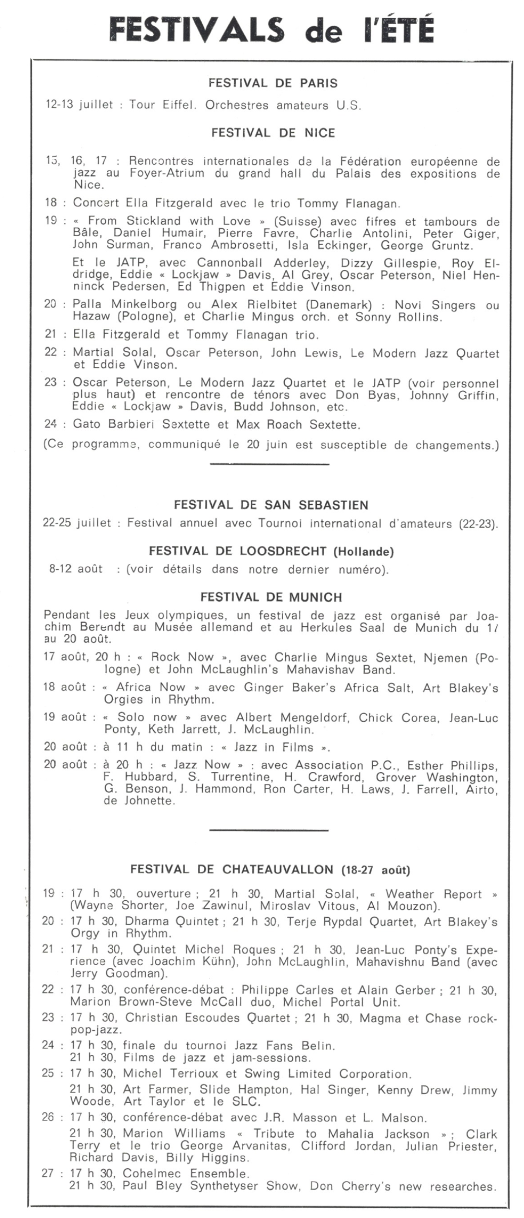
\includegraphics[width=\linewidth,keepaspectratio]{JH_Program_07_72.png}
		\caption{Programme de festival extrait de \textit{Jazz Hot}, juillet 1972.}
		\vspace{-1.1cm}
		\label{fig:jazzhot_program}
	\end{wrapfigure}
    expressions régulières adaptées à la structure des encarts de concerts et de festivals dans \textit{Jazz Hot} (Fig.~\ref{fig:jazzhot_program}). Cette méthode a permis de relever systématiquement le nom de l'artiste, le lieu et la date de performance. Un travail manuel de vérification a ensuite été mené pour corriger les faux positifs issus du script et pour enrichir la base par l'identification des musiciens associés au free jazz.
    La base de données qui en résulte comprend 10 364 entrées réparties entre 3593 artistes et 372 villes uniques et suit une structure événementielle où chaque ligne correspond à la participation d'un artiste à un événement donné. 
    Pour d’obtenir les coordonnées géographiques nécessaires à la cartographie, les villes mentionnées dans la base ont ensuite été réconciliées avec Wikidata. Ce choix répond à une contrainte du corpus puisque à peine 30 \% des entrées comportent une adresse complète. La contrepartie de cette décision est une perte de granularité spatiale, surtout pour Paris intra-muros où la diversité des clubs et des salles se trouve ramenée à un point unique. Cette limite appelle donc de futurs travaux à enrichir les adresses à partir de sources complémentaires.
	
	\subsection{Cartographie}
	La visualisation de données spatiotemporelles soulève des enjeux de lisibilité qui impliquent de sélectionner des modes de représentation accessibles. La solution présentée ici propose une plateforme réunissant plusieurs visualisations complémentaires qui permettent à l'utilisateur de naviguer entre différentes cartes et d'accéder directement à la base de données: \href{https://github.com/Jazz-Hot-Project}{https://jazz-hot-project.github.io/}. Cette démarche multiscalaire vise à offrir une granularité d'analyse en facilitant une exploration précise des cartes et des données.
    
    La première visualisation montre les réseaux de destinations sur toute la période étudiée avec l'épaisseur des traits et l'intensité des couleurs qui augmentent en fonction du nombre de trajets enregistrés (Fig.~\ref{fig:general_circuit_map}). Il convient toutefois de préciser que cette carte ne représente pas des parcours réels, mais le séquençage chronologique et spatial des entrées dans la base de données. Si certains enchaînements attestent d'un trajet effectif entre deux destinations, par exemple lorsque les dates se succèdent à un jour près, la visualisation relie plus généralement les destinations successives d'un artiste indépendamment de l'écart temporel qui les sépare.
    
    La seconde visualisation, centrée sur la France dans l'espace continental européen, représente des points dont le rayon varie proportionnellement au nombre de concerts joués dans chaque lieu (Fig.~\ref{fig:general_places_map}). Une visualisation spécifique au free jazz a enfin été produite montrant la proportion d'artistes free par rapport au nombre total de concerts dans chaque lieu à l'échelle de la France (Fig.~\ref{fig:free_jazz_proportion_map_general}), et de l'Île-de-France (Fig.~\ref{fig:free_jazz_proportion_map_idf}).
	
		\begin{figure}[ht]
		\centering
		\begin{minipage}[t]{0.48\linewidth}
			\centering
			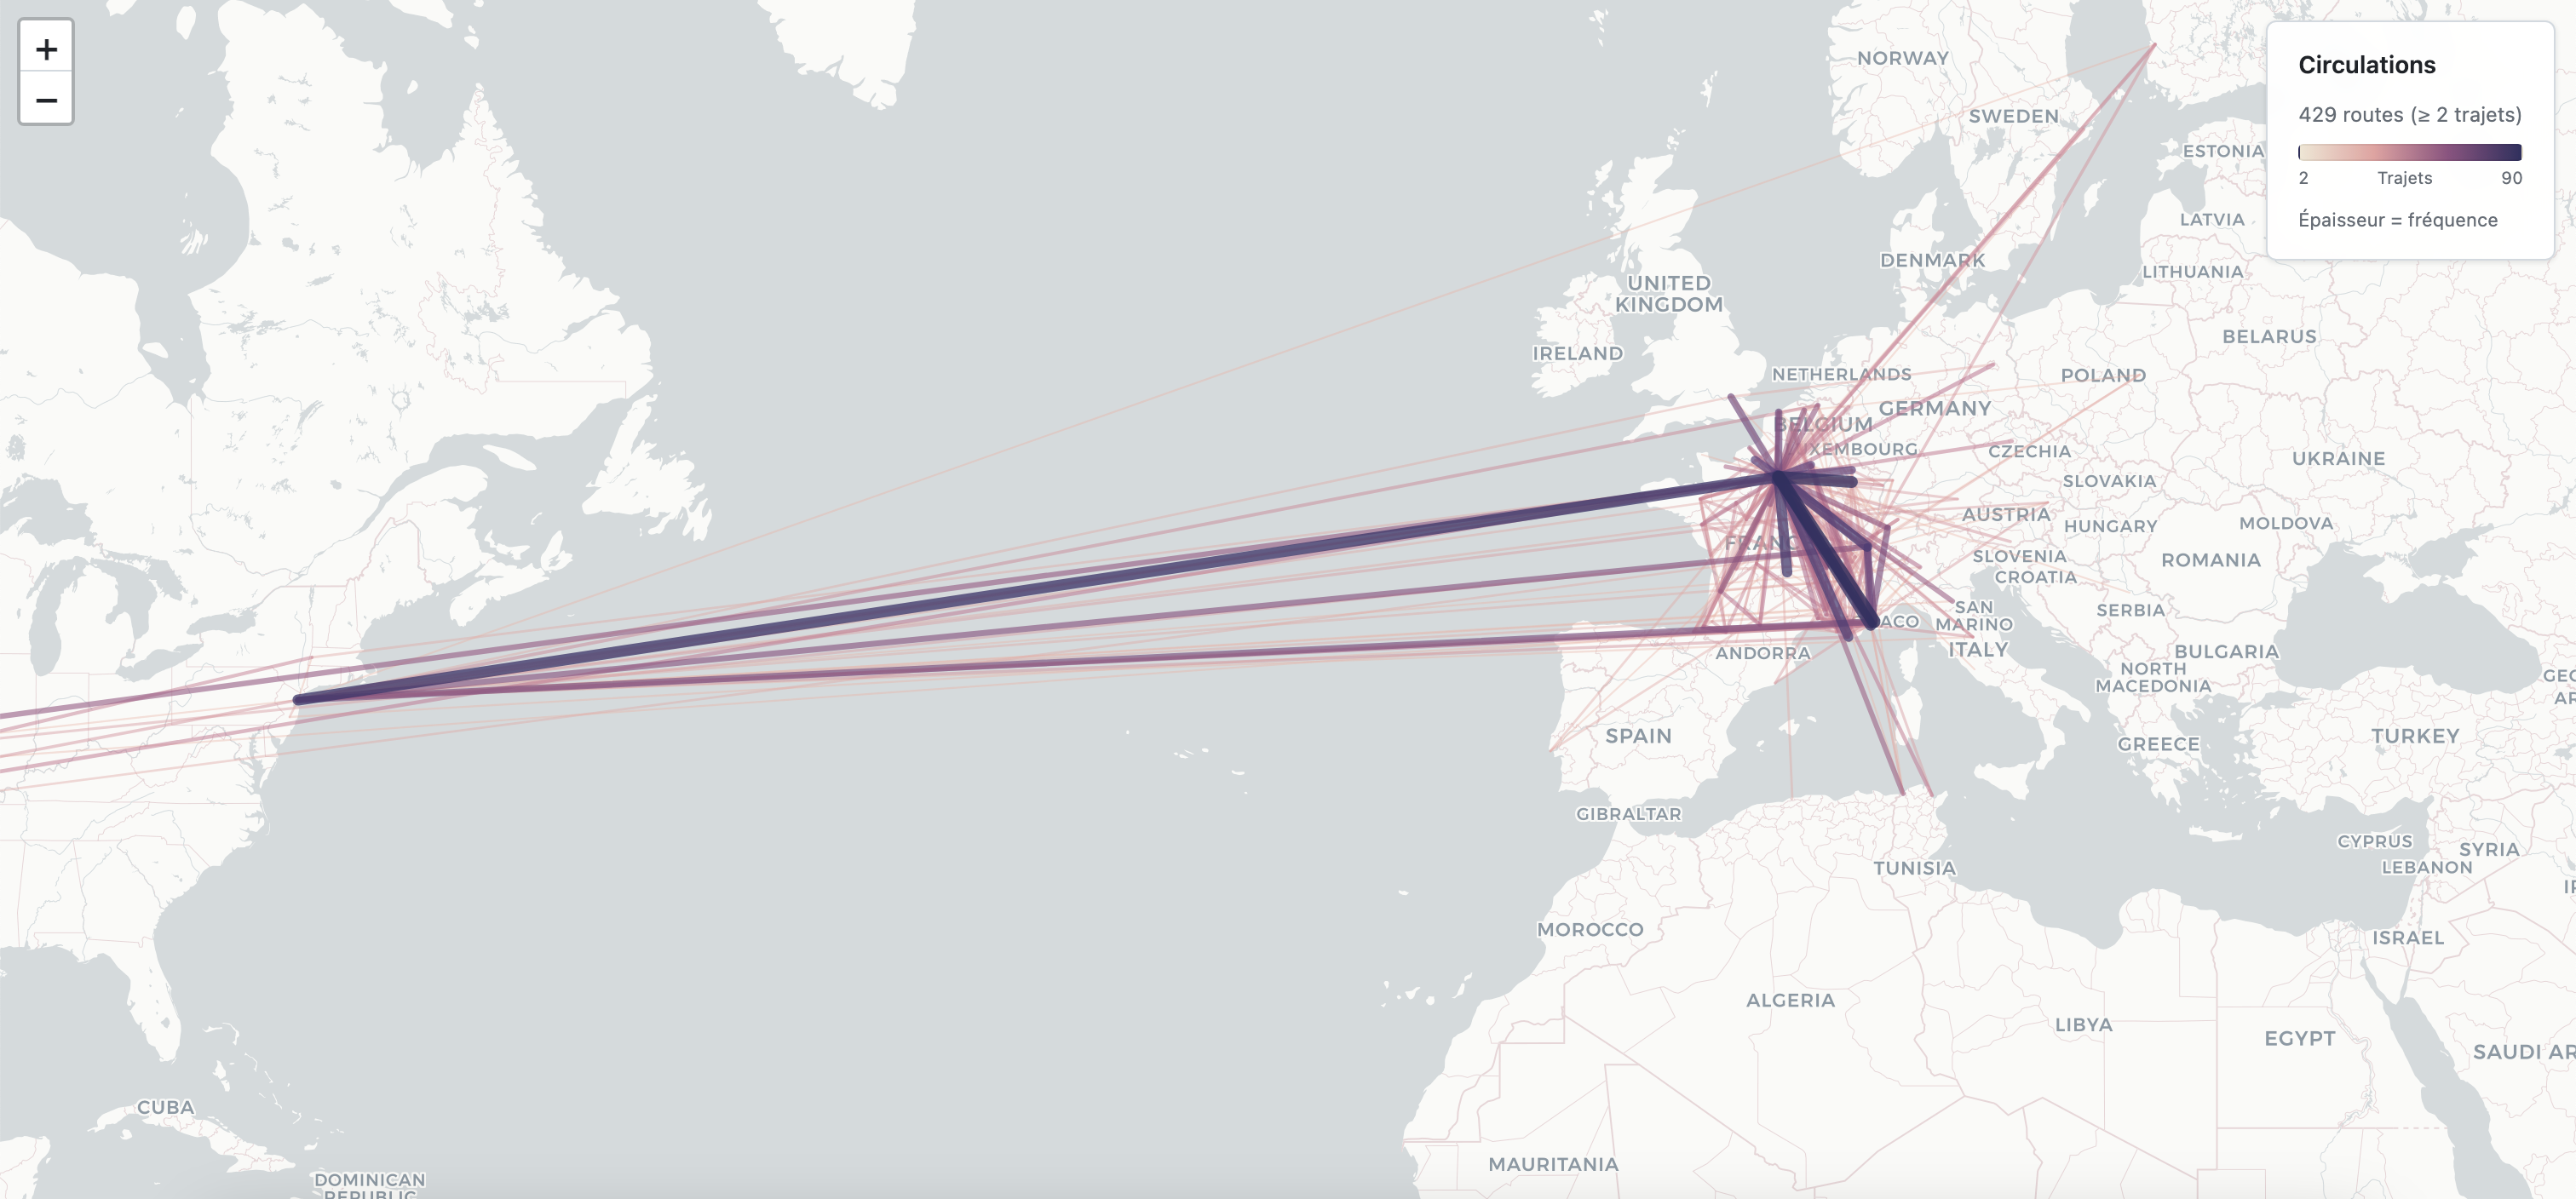
\includegraphics[width=\linewidth]{General_Circuit_festivals.png}
			\caption{Fréquence des itinéraires à échelle transatlantique (1966-1976).}
			\label{fig:general_circuit_map}
		\end{minipage}
		\hfill
		\begin{minipage}[t]{0.48\linewidth}
			\centering
			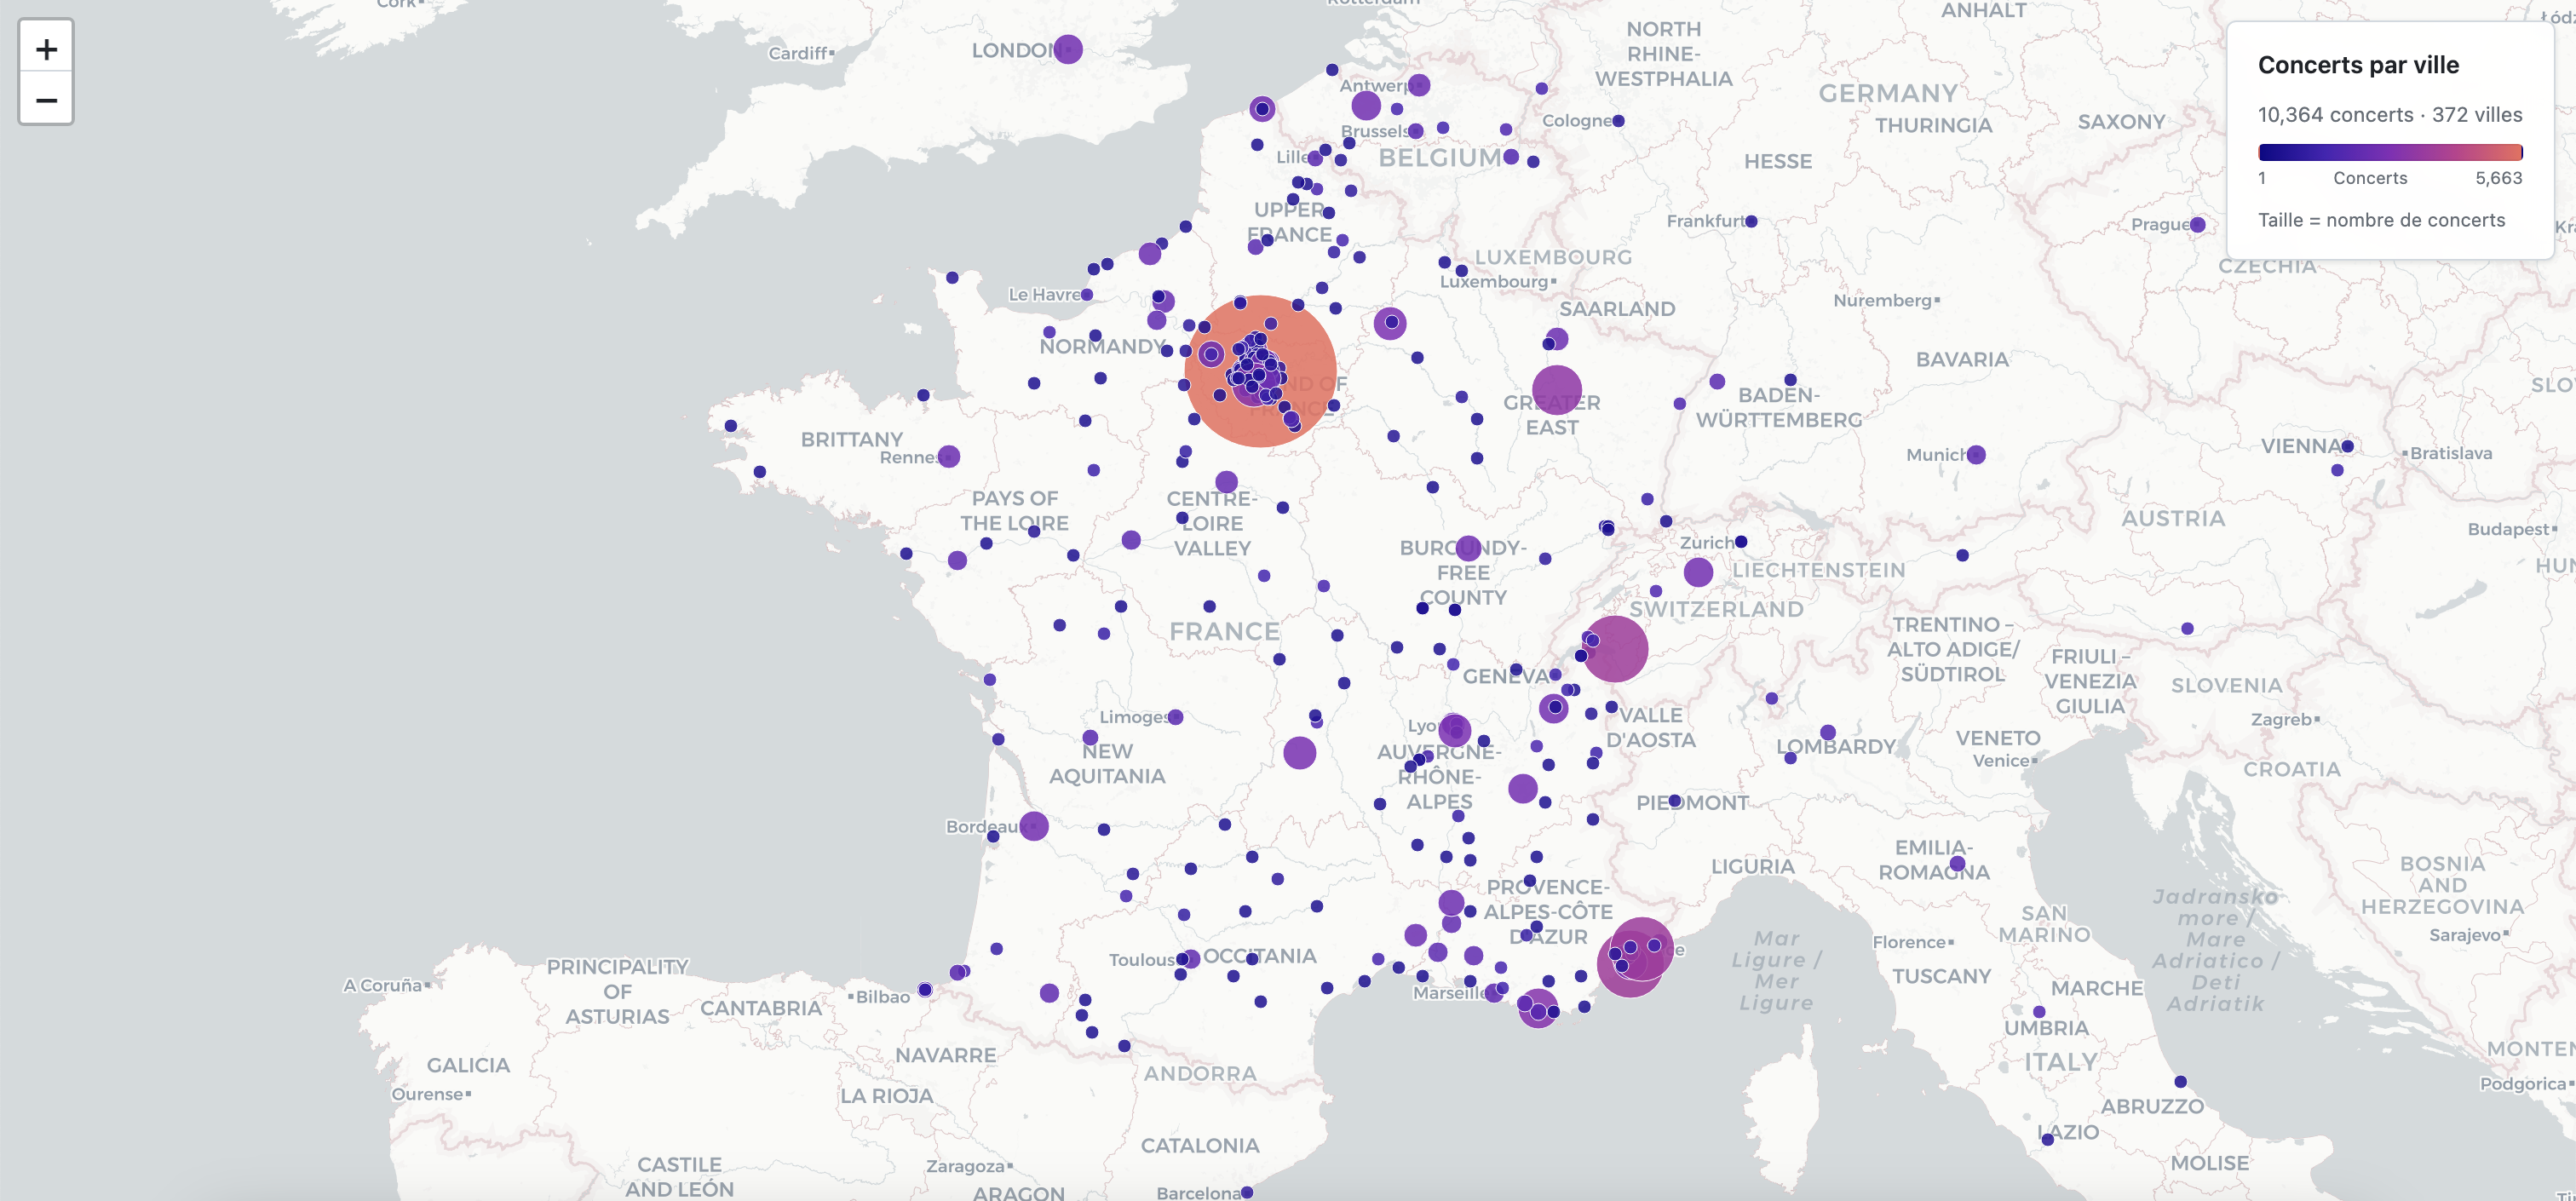
\includegraphics[width=\linewidth]{General_points_villes_circuit_festival.png}
			\caption{Lieux de représentations scéniques à échelle européenne (1966-1976).}
			\label{fig:general_places_map}
		\end{minipage}
	\end{figure}
	
	\begin{figure}[ht]
		\centering
		\begin{minipage}[t]{0.48\linewidth}
			\centering
			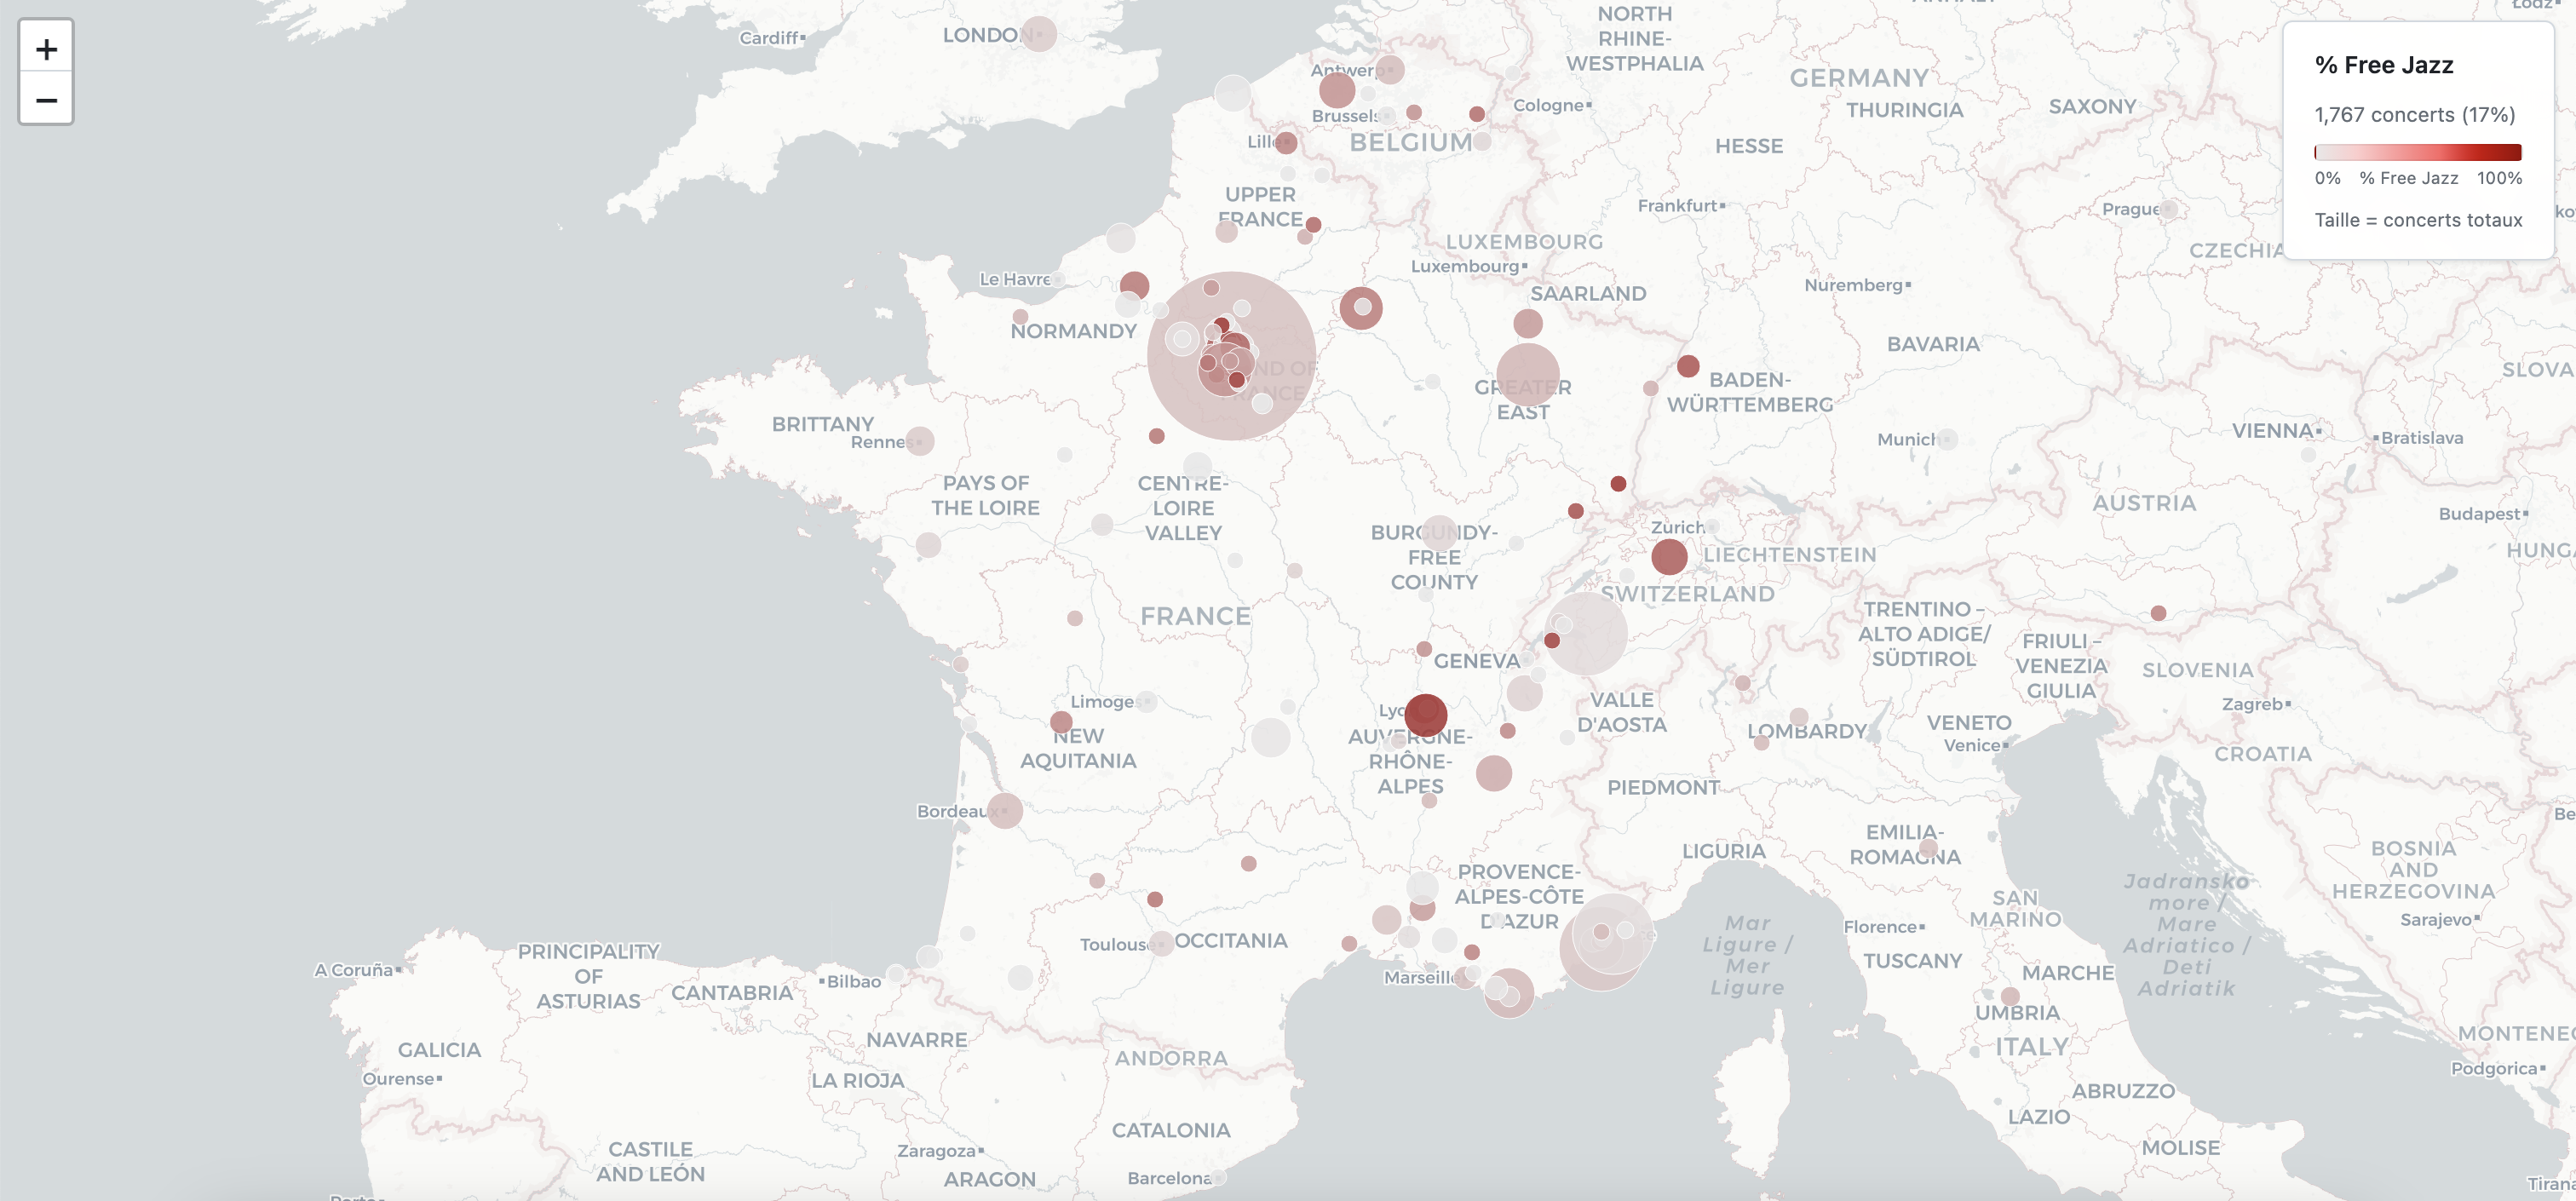
\includegraphics[width=\linewidth]{Carte_proportion free jazz concerts_general.png}
			\caption{Proportion du free jazz représenté sur le territoire européen francophone (1966-1976).}
			\label{fig:free_jazz_proportion_map_general}
		\end{minipage}
		\hfill 
		\begin{minipage}[t]{0.48\linewidth}
			\centering
			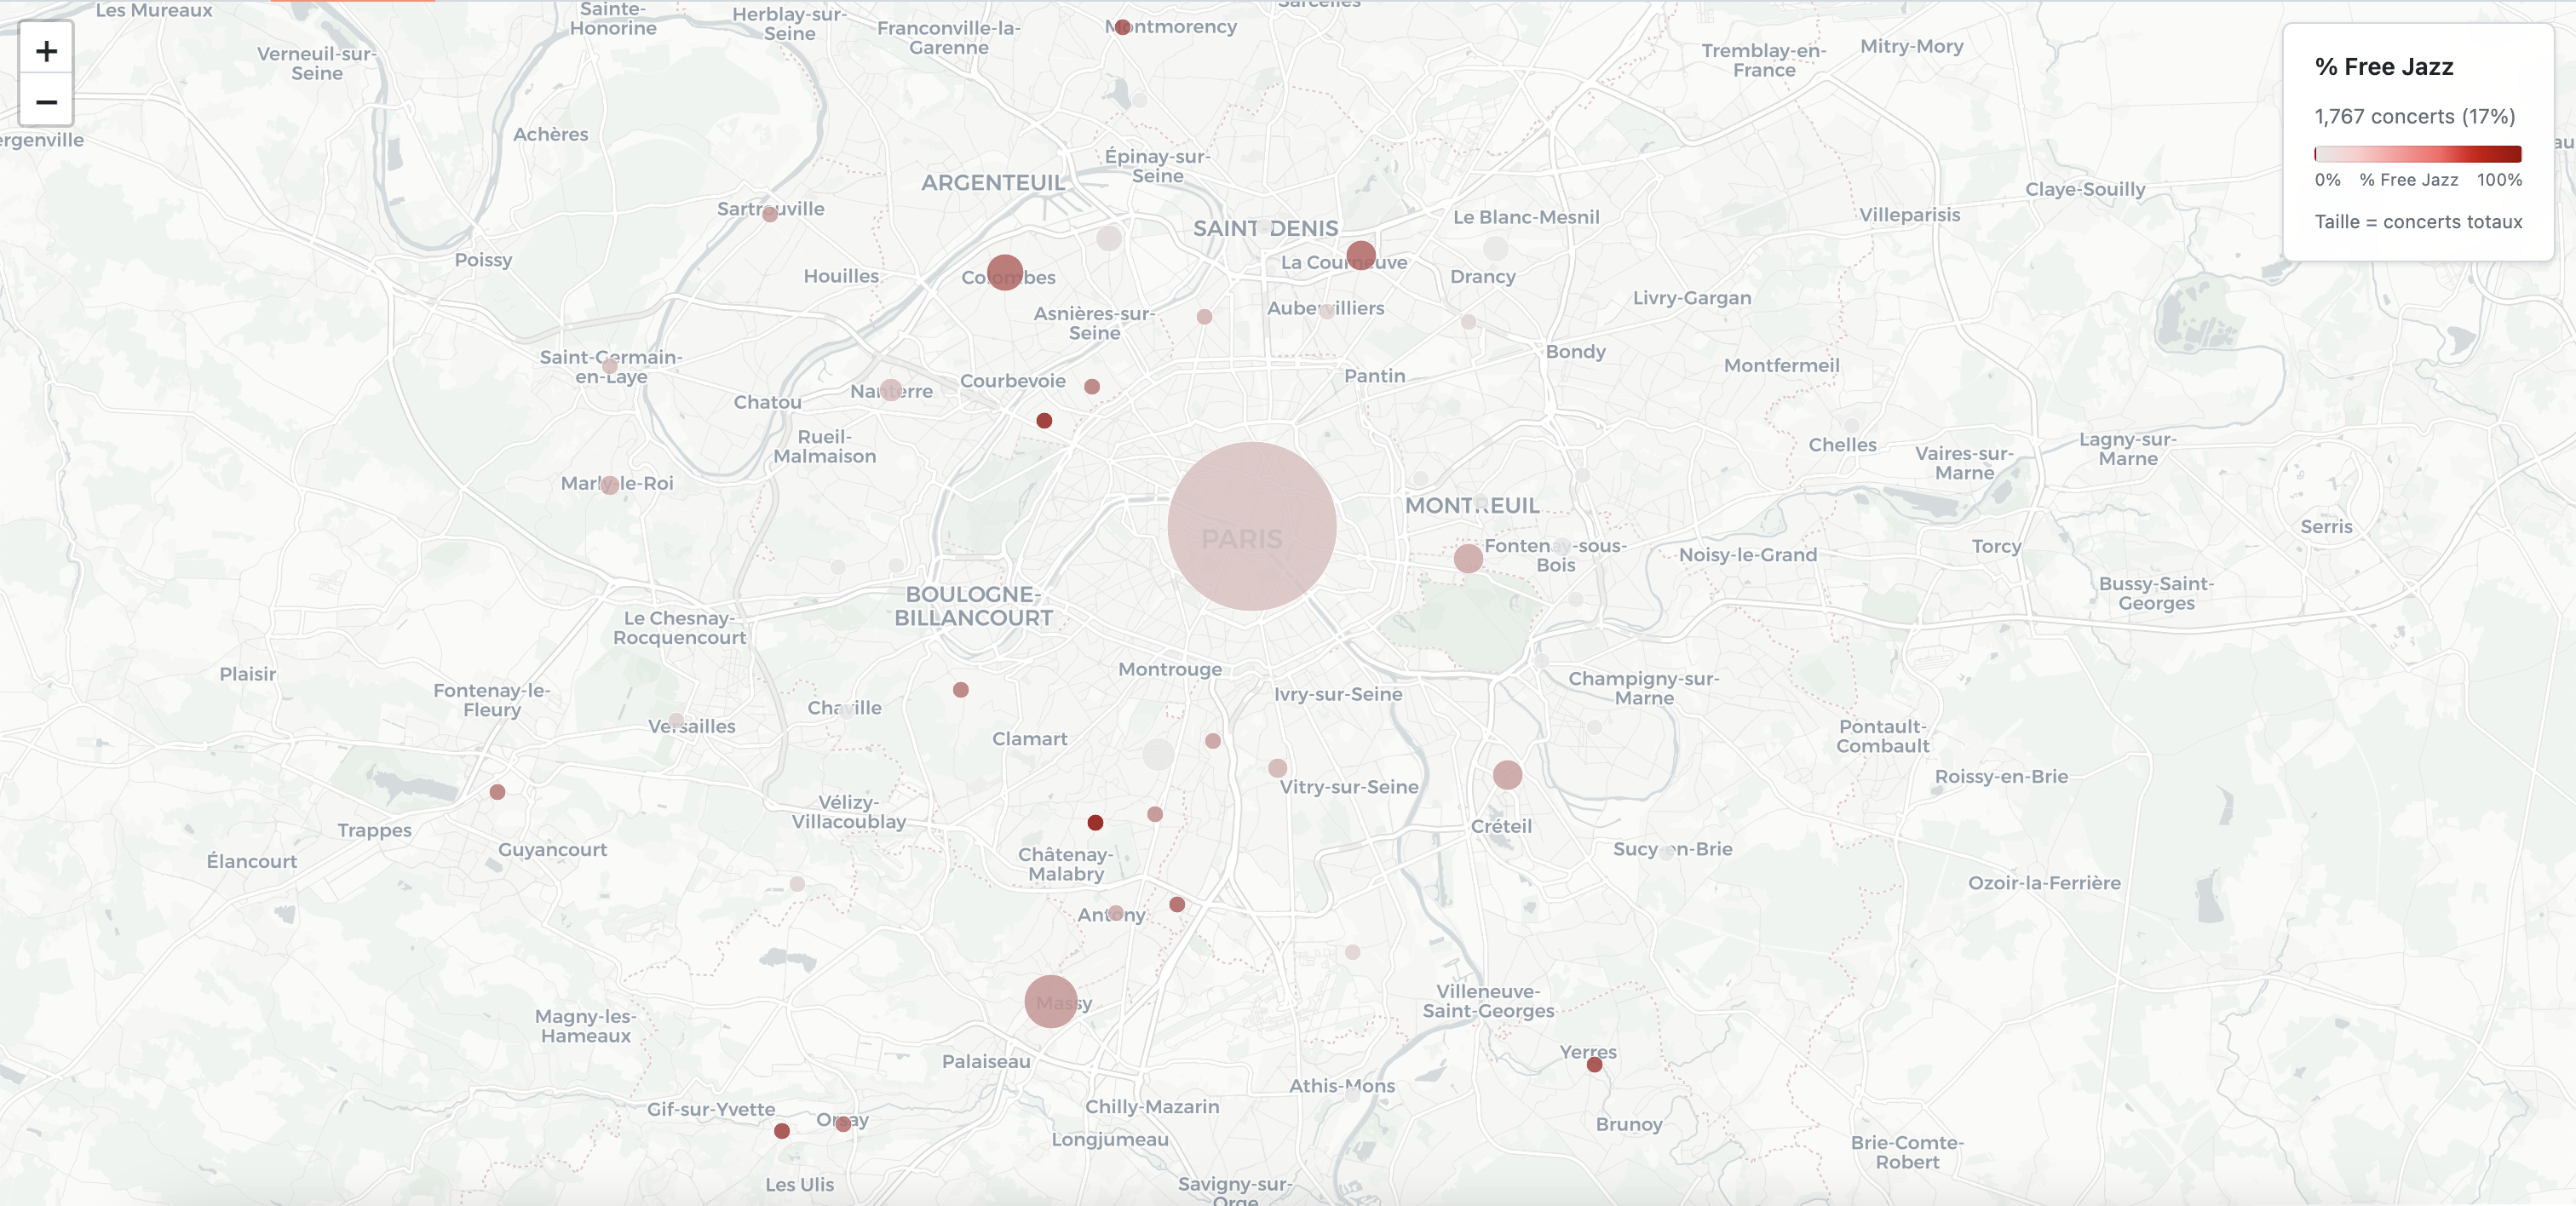
\includegraphics[width=\linewidth]{Carte_proportion free jazz concerts_IDF.png}
			\caption{Proportion du free jazz représenté en Île-de-France (1966-1976).}
			\label{fig:free_jazz_proportion_map_idf}
		\end{minipage}
		\vspace{-.5cm}
	\end{figure}
	
	\section{Discussion}
    Ces premiers relevés cristallise les traces morcelées des jazzmen sur le territoire francophone. En effet, les artères principales dessinent un parcours privilégié par les artistes, où un axe transatlantique entre Paris et New York affirme un canal déjà ancien (Fig.~\ref{fig:general_circuit_map}). La position centrale de Paris est toutefois nuancée par l'importance des festivals d'été à Montreux (Suisse), Nice et Antibes/Juan-les-Pins qui forment le réseau principal avec la capitale \footnote{Dans une moindre mesure, le circuit s'étend aux festivals de Châteauvallon (Toulon), Nancy et Super-Besse (Massif central).} (Fig.~\ref{fig:General_points_villes_circuit_festival}). Nos données montrent que ce réseau profite d'abord aux artistes établis comme Dizzy Gillespie, Clark Terry ou Charles Mingus \footnote{plus de 70 \% de leurs apparitions sont en festival sur la période.}, parcourant l'Europe forts de leur succès des décennies précédentes. Ce circuit suggère que les festivals de jazz structurent la diffusion de cette musique sur le territoire et que les flux de jazzmen résultent avant tout de l'économie de la tournée et des opportunités qu'offre le marché européen. Apparu en France dès les années 1940, le modèle du festival international de jazz repose d'abord sur l'invitation de joueurs américains de renom avant la programmation d'artistes émergents d'Europe ou d'ailleurs \cite{mckay_festivals_2018}. En parallèle, le déclin de la demande américaine pour le jazz dans les années 1960 conduit un nombre croissant de musiciens à venir jouer en France, où certains s'y installent durablement. Sunny Murray, Marion Brown, Steve Lacy, Noah Howard ou Frank Wright traversent l'Atlantique attirés par la perspective d'une meilleure réception de leur musique, dans un pays dont la réputation d'accueil envers les jazzmen était déjà établie \cite{drott_free_2008}. Festivals et scène parisienne fonctionnent ainsi comme des espaces de rencontres professionnelles et musicales offrant aux artistes des opportunités de rejoindre une formation, de toucher un public plus large \cite{mckay_festivals_2018} ou de décrocher un contrat d'enregistrement \cite{drott_free_2008}. Nos projections illustrent ainsi la centralité de ces pôles, qui constituent pour les artistes un enjeu à la fois économique et symbolique de visibilité et de reconnaissance \cite{picaud_comment_2017}.

    Ces cartes mettent également en évidence un réseau sous-jacent propre au free jazz. En observant la part du free jazz dans le total des concerts par ville, nous constatons qu'il ne recoupe qu'en partie le réseau principal et se déploie davantage en banlieue et en province, autour de lieux dédiés comme Willisau (Suisse), Saint-Fons ou l'American Center de Paris. En dépit de sa marginalité, il est documenté sur l'ensemble du territoire français, dessinant un réseau alternatif au circuit classique. Pour comprendre ce déploiement parallèle, il est nécessaire d'interroger la source qui le relaie et le contexte éditorial dans lequel elle s'inscrit. Au tournant des années 1960, une nouvelle génération de critiques \footnote{dont Michel Le Bris qui prend la tête de la rédaction de Jazz Hot en 1968} qui embrasse le free jazz dans sa dimension contestataire et lui attribue des valeurs militantes  en accord avec la pensée anticoloniale de mai 68 \cite{drott_free_2008}. La répartition du free sur nos cartes est ainsi tributaire de cette ligne éditoriale qui conteste les centres et valorise les périphéries, d'autant plus qu'une partie de la rédaction organisait ou participait elle-même à certains de ces événements \cite{roueff_espace_2019}.
    
    Par ailleurs, la répartition entre artistes américains et européens sur ce réseau confirme que le free jazz s'inscrit dans une dynamique plus locale. La présence américaine est en effet minoritaire sur ce circuit \footnote{ environ 20 \% des artistes sur ce circuits sont américains}, et les artistes les plus actifs, comme Cecil Taylor ou Sun Ra, avaient pour la plupart déjà connu un succès à New York au début des années 1960, les rattachant davantage au modèle du réseau principal. Ainsi, ces cartes semblent plutôt témoigner de l'affirmation d'une scène européenne de musique improvisée. Un goût esthétique et idéologique s'est développé pour ce style, et des écosystèmes culturels se sont constitués aussi bien pour cultiver ces musiques dans des espaces locaux (événements militants, petits festivals, salles communales, MJC...) que pour inviter les précurseurs et les expatriés américains. L'absence de visualisation en frise chronologique nous retient toutefois de restituer avec précision les différentes phases que Jedediah Sklower identifie dans ce processus comme d'abord une découverte esthétique au début des années 1960, durant laquelle la présence du free sur nos cartes serait encore faible, puis une politisation au tournant des années 1970, marquée par une première diffusion portée principalement par les musiciens américains, enfin un détachement progressif de la culture afro-américaine dans la décennie suivante, où l'on observerait la scène européenne s'imposer sur l'ensemble du territoire \cite{sklower_free_2006}.

	\section{Pistes}
    Ce premier dépouillement ouvre plusieurs pistes d'approfondissement. La chaîne de traitement des données s'avère fonctionnelle mais reste perfectible à chaque étape, surtout au niveau de la segmentation des images et de l’automatisation de l’extraction des données. Pour aller plus loin, il conviendrait aussi de compléter les sources en intégrant davantage de revues et d'élargir le corpus à l'échelle européenne, ce qui supposerait toutefois une numérisation massive et l'entraînement de nouveaux modèles OCR adaptés aux imprimés en différentes langues.
    En outre, l'application gagnerait à être enrichie de nouvelles visualisations et en particulier d'une \textit{timeline} permettant de dégager des dynamiques d'évolution avec plus grande précision. Il resterait alors à mener une interrogation plus fine de la géographie du free jazz dans le temps : quels artistes jouent quelles musiques, dans quels espaces, et dans quelle mesure cela participe-t-il à la diffusion et à la réception de cette pratique ?

\section*{Données}

Application: \url{https://jazz-hot-project.github.io}

\noindent Github: \url{https://github.com/Jazz-Hot-Project}

\noindent Zenodo: \url{https://zenodo.org/records/18865177}
    
	
	% Imprime la bibliographie à la fin. Gardez cette ligne après le texte
	% principal de votre article et avant une annexe.
	\printbibliography	
	% Vous pouvez inclure une annexe en utilisant la commande suivante
	%\appendix
	
	%\section{Première section de l'annexe} \label{appdx:first}
	
	%Des annexes facultatives peuvent être ajoutées après la section des références. 
	
\end{document}